\documentclass[11pt,a4paper]{article}
\usepackage[utf8]{inputenc}
\usepackage[margin=2.4cm]{geometry}
\usepackage{amsmath,amssymb}
\usepackage{booktabs}
\usepackage{xcolor}
\usepackage{graphicx}
\usepackage{listings}
\usepackage{enumitem}
\usepackage{microtype}
\usepackage[colorlinks=true,linkcolor=blue!50!black,urlcolor=blue!50!black]{hyperref}

\definecolor{codegray}{gray}{0.45}
\definecolor{codeblue}{rgb}{0.1,0.2,0.6}
\lstset{
  language=Python,
  basicstyle=\ttfamily\footnotesize,
  keywordstyle=\color{codeblue},
  commentstyle=\color{codegray}\itshape,
  stringstyle=\color{teal},
  showstringspaces=false,
  breaklines=true,
  frame=single,
  rulecolor=\color{black!25},
  numbers=left,
  numberstyle=\tiny\color{codegray},
  literate={θ}{$\theta$}1 {ξ}{$\xi$}1,
}

\newcommand{\session}[3]{%
  \title{\textbf{#1}\\[2pt]\large #2}
  \author{astro-lab \,--\, #3}
  \date{}
  \maketitle
  \vspace{-1.5em}
}
\newcommand{\todo}[1]{\textcolor{red!60!black}{\textbf{[#1]}}}
\usepackage{framed}
\newenvironment{keyidea}{%
  \def\FrameCommand{\color{blue!40!black}\vrule width 2.5pt\hspace{8pt}\color{black}}%
  \MakeFramed{\advance\hsize-\width\FrameRestore}}{\endMakeFramed}

\newcommand{\dd}{\mathrm{d}}
\newcommand{\pc}{\,\mathrm{pc}}
\newcommand{\Msun}{M_\odot}
\newcommand{\Rsun}{R_\odot}
\setlist[itemize]{itemsep=2pt,topsep=4pt}
\setlist[enumerate]{itemsep=3pt,topsep=4pt}
\setlength{\parindent}{0pt}
\setlength{\parskip}{6pt}

\begin{document}
\session{Session 2: Orbits and Numerical Integration}{Two-body motion, leapfrog versus RK4, energy conservation}{reading notes}

\section*{Goals}
Understand why a symplectic integrator is the default for long gravitational simulations, and verify it by measuring energy error on an eccentric Kepler orbit.

\section{The two-body problem}
Two masses interact through $\mathbf F = -Gm_1m_2\,\hat{\mathbf r}/r^2$. In the centre-of-mass frame the problem reduces to one body of reduced mass $\mu$ moving in a central potential. We work in units $GM=1$, so a test particle obeys
\[
\ddot{\mathbf r} = -\frac{\mathbf r}{|\mathbf r|^{3}} .
\]
Two quantities are conserved exactly:
\[
E = \tfrac12 v^2 - \frac1r, \qquad \mathbf L = \mathbf r\times\mathbf v .
\]
A numerical method is judged by how well it preserves them over many orbits.

\section{Setting up an eccentric orbit}
With semi-major axis $a=1$ and eccentricity $e$, start at pericentre:
\[
r_p = a(1-e), \qquad v_p = \sqrt{\frac{1+e}{1-e}} \quad (GM=a=1).
\]
Then $E=-1/(2a)=-1/2$ and the period is $P=2\pi$. The script uses $e=0.6$, which is eccentric enough to stress a fixed timestep at pericentre.

\section{Two integrators}
\subsection*{Leapfrog (kick--drift--kick)}
\[
\mathbf v_{n+1/2} = \mathbf v_n + \tfrac{\Delta t}{2}\mathbf a(\mathbf r_n),\quad
\mathbf r_{n+1} = \mathbf r_n + \Delta t\,\mathbf v_{n+1/2},\quad
\mathbf v_{n+1} = \mathbf v_{n+1/2} + \tfrac{\Delta t}{2}\mathbf a(\mathbf r_{n+1}).
\]
It is second order, time-reversible and \emph{symplectic}: it exactly conserves a nearby ``shadow'' Hamiltonian $\tilde H = H + O(\Delta t^2)$. So the energy error oscillates and stays bounded instead of growing.

\subsection*{Classical RK4}
Fourth order and much more accurate per step, but not symplectic. Its energy error grows secularly because each step adds a small systematic error that does not cancel.

\begin{keyidea}
\textbf{Key idea.} Per-step accuracy and long-term behaviour are different properties. RK4 wins at small $\Delta t$ over short runs; leapfrog wins when the run is long enough for RK4's drift to accumulate.
\end{keyidea}

\section{Results from the repository script}
Measured with \texttt{kepler\_integrators.py}, $e=0.6$:
\begin{center}
\begin{tabular}{@{}lcrr@{}}
\toprule
Setting & Orbits & Leapfrog $\max|\Delta E/E|$ & RK4 $\max|\Delta E/E|$ \\ \midrule
$\Delta t=0.01$ & 100 & $7.4\times10^{-4}$ & $2.2\times10^{-6}$ \\
$\Delta t=0.05$ & 1000 & $1.9\times10^{-2}$ & $6.9\times10^{-2}$ \\
\bottomrule
\end{tabular}
\end{center}
At $\Delta t=0.01$ RK4 is better. At $\Delta t=0.05$ the leapfrog error stays flat at about $1.9\times10^{-2}$. In a separate 300-orbit run at the same $\Delta t$, RK4's error grew from $2.1\times10^{-3}$ in the first tenth of the run to $2.0\times10^{-2}$ in the last tenth, and by 1000 orbits it reached $6.9\times10^{-2}$. The figure \texttt{energy\_drift.png} in the repository shows the per-orbit maximum error for the 1000-orbit run.

\begin{center}
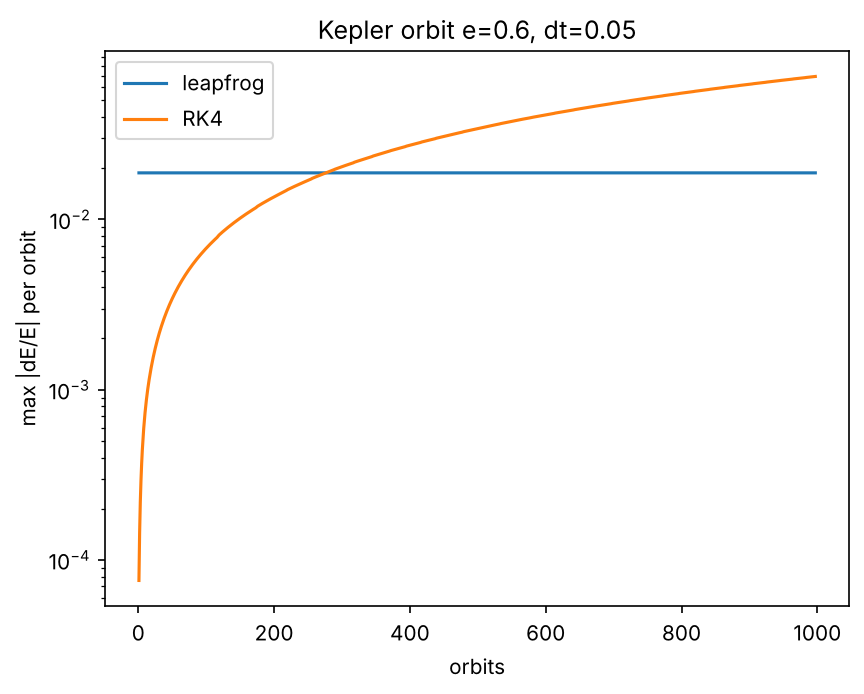
\includegraphics[width=0.62\linewidth]{../02_orbits/energy_drift.png}
\end{center}

\section{Code walkthrough}
\lstinputlisting{../02_orbits/kepler_integrators.py}

\section{Exercises}
\begin{enumerate}
\item Find the $\Delta t$ at which the two curves cross after 1000 orbits. How does it change with $e$?
\item Measure $|\mathbf L-\mathbf L_0|$ for both methods. Leapfrog conserves it to round-off for any central force: show why (the kick changes $\mathbf v$ by a vector parallel to $\mathbf r$, and the drift changes $\mathbf r$ by a vector parallel to $\mathbf v$). RK4 does not; explain what you see.
\item Implement the fourth-order Yoshida composition of leapfrog and compare with RK4.
\item Replace the fixed step with $\Delta t\propto r^{3/2}$ and describe what happens to leapfrog's energy error. (Hint: a variable step breaks symplecticity unless done carefully.)
\item Run the same setup with REBOUND (\texttt{WHFast} and \texttt{IAS15}) and compare.
\end{enumerate}

\section*{References}
\begin{itemize}
\item Hairer, Lubich, Wanner, \textit{Geometric Numerical Integration}, ch.\ I and IX
\item Rein \& Liu (2012), REBOUND, \textit{A\&A} 537, A128
\item Rein \& Tamayo (2015), WHFast, \textit{MNRAS} 452, 376
\end{itemize}
\end{document}
